\documentclass[11pt]{article}
% Time-stamp: <homework-02.tex, saved on Fri, Sep 14, 2007 at 12:46pm>
\usepackage[margin=1in, head=1in]{geometry}
\usepackage{amsmath, amssymb, amsthm}
\usepackage{fancyhdr}
\usepackage{graphicx}
\usepackage{pgfplots}

%\usepackage{pdfsync}
\addtolength{\textwidth}{.5in}
\addtolength{\leftmargin}{-1in}
\addtolength{\textheight}{.5in}
\addtolength{\topmargin}{-0.5in}

%\pagestyle{fancy}
%\lhead{MATH 200X }
%\chead{Fall 2007}
%\rhead{FINAL EXAM}
%\lfoot{}
%\cfoot{\thepage}
%\rfoot{}

\setcounter{secnumdepth}{0}
%\renewcommand{\theenumi}{\alph{enumi}}
%\renewcommand{\emptyset}{\varnothing}
\newcommand{\R}{\mathbb{R}}
\newcommand{\N}{\mathbb{N}}
\newcommand{\Z}{\mathbb{Z}}
\newcommand{\clm}{\par\textit{Claim:}\par}
\newcommand{\diam}{\mathrm{diam}}
\newcommand{\sect}{\textsection}

\parindent=0in
\parskip=0.5\baselineskip

\begin{document} 

\begin{center}MATH 156: Precalculus  \\ Fall 2015 \\ Worksheet \sect 2.8: One-to-One Functions and their Inverses\end{center}

\hrulefill

Here are the skills you want to have at the end of this section.
\begin{enumerate}
\item Be able to identify whether a given function is one-to-one or not {\emph{and explain your answer rigorously}} whether the function is given graphically or algebraically.
\item Be able to use the {\it{Inverse Function Property}} to show two functions are inverses of each other.
\item Be able to find the inverse of a given (one-to-one) function whether the function is given algebraically or graphically -- even in the instances in which the domain is restricted or you will need to restrict the domain.
\item Be able to interpret functions and their inverses in applied problems. 
\end{enumerate}

\hrulefill

\begin{enumerate}
\item For each function below (two given as graphs and two given algebraically) determine whether or not the function is one-to-one and explain your answer. If the function is given algebraically, give an algebraic explanation.
\begin{enumerate}
%graph1
\item $h(x)$ 
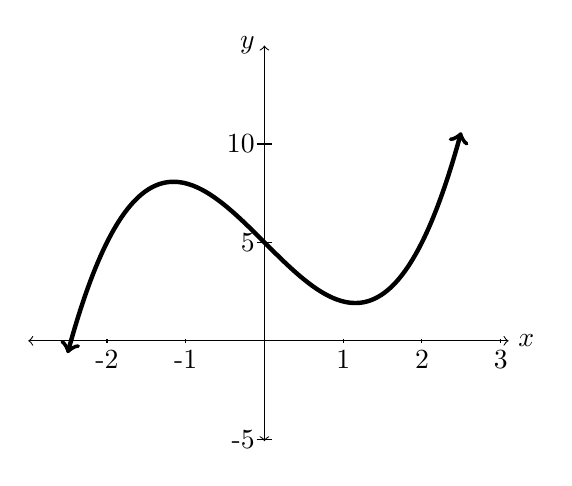
\begin{tikzpicture}[baseline=(current bounding box.center), xscale=1, yscale=.25]
\draw[<->] (0,-5.1) -- (0,15) node[left] {$y$};
\draw[<->](-3,0) -- (3.1, 0) node[right] {$x$};
\foreach \i in {-2,-1, 1, 2,3,}{\draw (\i, .1) -- (\i, -.1);
\draw (\i,0) node[below] {\i};
}
\foreach \i in {-5,5,10}{
\draw (-.1, \i) -- (.1,\i);
\draw (0,\i) node[  left] {\i};
}
\draw[smooth,samples=200,domain=-2.5:2.5, ultra thick,,<->]  plot({\x},{\x^3-4*\x+5});
\end{tikzpicture}
%graph2
\item $g(x)$
\begin{tikzpicture}[baseline=(current bounding box.center), xscale=1, yscale=1]
\draw[<->] (0,-1) -- (0,5) node[left] {$y$};
\draw[<->](-1,0) -- (5, 0) node[right] {$x$};
\foreach \i in { 1, 2,3,}{\draw (\i, .1) -- (\i, -.1);
\draw (\i,0) node[below] {\i};
}
\foreach \i in {1,2,3}{
\draw (-.1, \i) -- (.1,\i);
\draw (0,\i) node[  left] {\i};
}
\draw[smooth,samples=200,domain=.3:3.5, ultra thick,,<->]  plot({\x},{1/\x});
\end{tikzpicture}
%function1
\item $f(x)=\sqrt{x-3}$
\vfill
%function2
\item $g(x)=x^6+4$
\vfill
\end{enumerate}

\item Use the Inverse Function Property to show that $f=x^3-1$ and $g=\sqrt[3]{x+1}$ are inverses of each other.
\vfill

\newpage

\item Find the inverses of the functions below. For functions given algebraically, give the inverse algebraically. For functions given graphically, give the inverse graphically. Note the third example has a restricted domain. For the fourth example, you will have to restrict the domain appropriately. (Yes, there is more than one option here.)
\begin{enumerate}
\item $f(x)= \frac{3-4x}{8x-1}$

\vfill

\item $g(x)$
\begin{tikzpicture}[baseline=(current bounding box.center), xscale=1, yscale=1]
\draw[<->] (0,-2) -- (0,5) node[left] {$y$};
\draw[<->](-2,0) -- (5, 0) node[right] {$x$};
\foreach \i in { -1,1, 2,3,4}{\draw (\i, .1) -- (\i, -.1);
\draw (\i,0) node[below] {\i};
}
\foreach \i in {-1,1, 2,3,4}{
\draw (-.1, \i) -- (.1,\i);
\draw (0,\i) node[  left] {\i};
}
\draw[smooth,samples=200,domain=-1:1, ultra thick]  plot({\x},{2*\x+1});
\draw[smooth,samples=200,domain=1:3, ultra thick]  plot({\x},{\x/2+5/2});
\end{tikzpicture}

\vfill

\item $g(x)=x^2+x$ for $x\geq -1/2$\\
\vfill

\newpage

\item $g(x)$
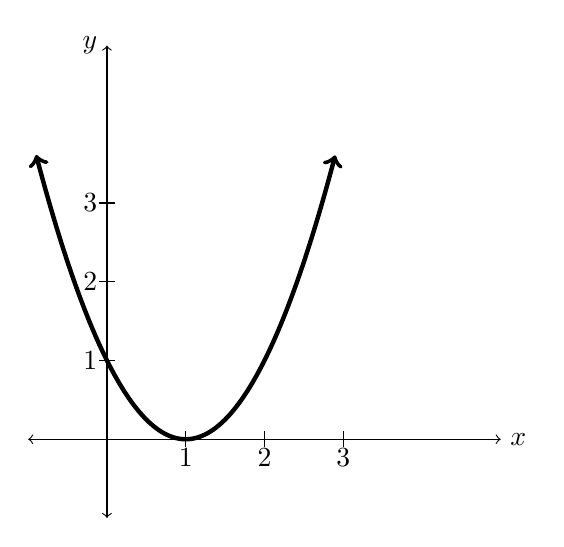
\begin{tikzpicture}[baseline=(current bounding box.center), xscale=1, yscale=1]
\draw[<->] (0,-1) -- (0,5) node[left] {$y$};
\draw[<->](-1,0) -- (5, 0) node[right] {$x$};
\foreach \i in { 1, 2,3,}{\draw (\i, .1) -- (\i, -.1);
\draw (\i,0) node[below] {\i};
}
\foreach \i in {1,2,3}{
\draw (-.1, \i) -- (.1,\i);
\draw (0,\i) node[  left] {\i};
}
\draw[smooth,samples=200,domain=-0.9:2.9, ultra thick,,<->]  plot({\x},{(\x -1)^2});
\end{tikzpicture}
\end{enumerate}
\vspace{.5in}


\item A tank holds 100 gallons of water which drains from a leak in the bottom causing the tank to empty in 40 minutes. According to Torricelli's Law, the volume $V$ of the water remaining in the tank after $t$ minutes is given by the function

$$V=100\left( 1-\frac{t}{40} \right)^2.$$
\begin{enumerate}
\item If we think of $V$ as a function of $t$ (that is, $V=f(t)$) if $f$ one-to-one? (Explain your answer).
\item Find the inverse of the function above and give it an appropriate name. 
\item What does this function you found in part c represent?
\item Find $f^{-1}(15)$ and explain what this number means.
\end{enumerate}

\vfill
\end{enumerate}
\end{document}

